\documentclass[man,floatsintext]{apa6}
\usepackage{lmodern}
\usepackage{amssymb,amsmath}
\usepackage{ifxetex,ifluatex}
\usepackage{fixltx2e} % provides \textsubscript
\ifnum 0\ifxetex 1\fi\ifluatex 1\fi=0 % if pdftex
  \usepackage[T1]{fontenc}
  \usepackage[utf8]{inputenc}
\else % if luatex or xelatex
  \ifxetex
    \usepackage{mathspec}
  \else
    \usepackage{fontspec}
  \fi
  \defaultfontfeatures{Ligatures=TeX,Scale=MatchLowercase}
\fi
% use upquote if available, for straight quotes in verbatim environments
\IfFileExists{upquote.sty}{\usepackage{upquote}}{}
% use microtype if available
\IfFileExists{microtype.sty}{%
\usepackage{microtype}
\UseMicrotypeSet[protrusion]{basicmath} % disable protrusion for tt fonts
}{}
\usepackage{hyperref}
\hypersetup{unicode=true,
            pdftitle={Both statistical and social information modulate children's eye movements during language comprehension and word learning},
            pdfauthor={Kyle MacDonald, Elizabeth Swanson, \& Michael C. Frank},
            pdfkeywords={eye movements; word learning; language comprehension;
information-seeking; gaze following},
            pdfborder={0 0 0},
            breaklinks=true}
\urlstyle{same}  % don't use monospace font for urls
\usepackage{graphicx,grffile}
\makeatletter
\def\maxwidth{\ifdim\Gin@nat@width>\linewidth\linewidth\else\Gin@nat@width\fi}
\def\maxheight{\ifdim\Gin@nat@height>\textheight\textheight\else\Gin@nat@height\fi}
\makeatother
% Scale images if necessary, so that they will not overflow the page
% margins by default, and it is still possible to overwrite the defaults
% using explicit options in \includegraphics[width, height, ...]{}
\setkeys{Gin}{width=\maxwidth,height=\maxheight,keepaspectratio}
\IfFileExists{parskip.sty}{%
\usepackage{parskip}
}{% else
\setlength{\parindent}{0pt}
\setlength{\parskip}{6pt plus 2pt minus 1pt}
}
\setlength{\emergencystretch}{3em}  % prevent overfull lines
\providecommand{\tightlist}{%
  \setlength{\itemsep}{0pt}\setlength{\parskip}{0pt}}
\setcounter{secnumdepth}{0}
% Redefines (sub)paragraphs to behave more like sections
\ifx\paragraph\undefined\else
\let\oldparagraph\paragraph
\renewcommand{\paragraph}[1]{\oldparagraph{#1}\mbox{}}
\fi
\ifx\subparagraph\undefined\else
\let\oldsubparagraph\subparagraph
\renewcommand{\subparagraph}[1]{\oldsubparagraph{#1}\mbox{}}
\fi

%%% Use protect on footnotes to avoid problems with footnotes in titles
\let\rmarkdownfootnote\footnote%
\def\footnote{\protect\rmarkdownfootnote}


  \title{Both statistical and social information modulate children's eye
movements during language comprehension and word learning}
    \author{Kyle MacDonald\textsuperscript{1}, Elizabeth Swanson\textsuperscript{1},
\& Michael C. Frank\textsuperscript{1}}
    \date{}
  
\shorttitle{Integrating social and statistical information}
\affiliation{
\vspace{0.5cm}
\textsuperscript{1} Stanford University}
\keywords{eye movements; word learning; language comprehension; information-seeking; gaze following\newline\indent Word count: X}
\usepackage{csquotes}
\usepackage{upgreek}
\captionsetup{font=singlespacing,justification=justified}

\usepackage{longtable}
\usepackage{lscape}
\usepackage{multirow}
\usepackage{tabularx}
\usepackage[flushleft]{threeparttable}
\usepackage{threeparttablex}

\newenvironment{lltable}{\begin{landscape}\begin{center}\begin{ThreePartTable}}{\end{ThreePartTable}\end{center}\end{landscape}}

\makeatletter
\newcommand\LastLTentrywidth{1em}
\newlength\longtablewidth
\setlength{\longtablewidth}{1in}
\newcommand{\getlongtablewidth}{\begingroup \ifcsname LT@\roman{LT@tables}\endcsname \global\longtablewidth=0pt \renewcommand{\LT@entry}[2]{\global\advance\longtablewidth by ##2\relax\gdef\LastLTentrywidth{##2}}\@nameuse{LT@\roman{LT@tables}} \fi \endgroup}

\authornote{

Correspondence concerning this article should be addressed to Kyle
MacDonald, 450 Serra Mall, Stanford, CA 94306. E-mail:
\href{mailto:kylem4@stanford.edu}{\nolinkurl{kylem4@stanford.edu}}}

\abstract{
Children process words in complex contexts that lend themselves to an in
principle unlimited number of possible interpretations. How do learners
find the correct lexicon? Statistical accounts propose that learning
unfolds via the aggregation of consistent word-object co-occurrences
over time. Social-pragamatic theories emphasize how grounded
interactions with social partners reduces ambiguity during individual
labeling events. Here, we present three studies of eye movements during
language processing that ask how learners intergrate statistical and
social information to shape real-time decisions about visual fixation.
First, both children (n=XXX) and adults (n=31) showed similar gaze
dynamics when processing familiar words that either did or did not occur
with an accompanied social cue to reference (eye gaze). Second, in a
minimal cross-situational word learning task, adults (n=XXX) allocated
more fixations and showed stronger memory for novel word-object mappings
that were learned in the presence of a social cue. Finally, in contrast
to the familiar word context, both children (n=XXX) and adults (n=XXX)
were slower to look away from a speaker's face when she was likely to
provide a gaze cue to disambiguate the meaning of a novel word. This
differential looking pattern increased over the course of the
experiment, as learners were exposed to more word-object co-occurrences
and gained experience with the speaker. Taken together, these results
show that decisions about how to seek visual information during language
acquisition are a function of the interaction of statistical and social
information.


}

\begin{document}
\maketitle

\hypertarget{introduction}{%
\section{Introduction}\label{introduction}}

\hypertarget{analytic-approach}{%
\section{Analytic approach}\label{analytic-approach}}

To quantify evidence for our predictions, we follow the analysis plan of
MacDonald, Marchman, Fernald, and Frank (2018) and present four
analyses: (1) the timecourse of listeners' looking to each area of
interest (AOI), (2) the Reaction Time (RT) and Accuracy of listeners'
first shifts away from the signer/speaker, (3) an Exponentially Weighted
Moving Average (EWMA) of first shifts, and (4) a Drift Diffusion Model
(DDM) of first shifts.\footnote{All analysis code can be found in the
  online repository for this project:
  \url{https://github.com/kemacdonald/speed-acc-novel}.}

First, we analyzed the timecourse of participants' looking to each AOI
in the visual scene as the target sentence unfolded. Proportion looking
reflects the mean proportion of trials on which participants fixated on
the speaker, the target image, or the distracter image at every 33-ms
interval of the stimulus sentence. We tested condition differences in
the proportion looking to the language source -- signer or speaker --
using a nonparametric cluster-based permutation analysis, which accounts
for the issue of taking multiple comparisons across many time bins in
the timecourse (Maris \& Oostenveld, 2007). A higher proportion of
looking to the language source in the gaze condition would indicate
listeners' prioritization of seeking visual information from the
speaker.

Next, we analyzed the RT and Accuracy of participants' initial gaze
shifts away from the speaker to objects. RT corresponds to the latency
of shifting gaze away from the central stimulus to either object
measured from the onset of the target noun. All reaction time
distributions were trimmed to between zero and two seconds and RTs were
modeled in log space. Accuracy corresponds to whether participants'
first gaze shift landed on the target or the distracter object. If
listeners generate slower but more accurate gaze shifts, this provides
evidence that gathering more visual information from the signer/speaker
led to more robust language comprehension.

We used the \texttt{rstanarm} (Gabry \& Goodrich, 2016) package to fit
Bayesian mixed-effects regression models. The mixed-effects approach
allowed us to model the nested structure of our data -- multiple trials
for each participant and item, and a within-participants manipulation --
by including random intercepts for each participant and item, and a
random slope for each item and gaze condition. We used Bayesian
estimation to quantify uncertainty in our point estimates, which we
communicate using a 95\% Highest Density Interval (HDI). The HDI
provides a range of credible values given the data and model.

Following the behavioral results, we present two model-based
analyses.\footnote{For more details about the model-based analyses see
  MacDonald et al. (2018)} The goal of each model is to move beyond a
description of the data and to map behavioral differences to underlying
psychological processes. The EWMA models changes in the tendency to
generate random gaze shifts as a function of RT (Vandekerckhove \&
Tuerlinckx, 2007). This model allows us to quantify the proportion of
gaze shifts that were classified as language-driven as opposed to
guessing. If listeners seek more visual information from the language
source, then they should generate a higher proportion of language-driven
shifts and fewer random responses.

Finally, following Vandekerckhove and Tuerlinckx (2007), we selected the
gaze shifts categorized as language-driven by the EWMA and fit a
hierarchical Bayesian Drift-Diffusion Model (HDDM) (Wiecki, Sofer, \&
Frank, 2013). The DDM is a cognitive model of decision making developed
over the past forty years (Ratcliff \& McKoon, 2008) that can quantify
differences in the underlying decision process that lead to different
patterns of observable behavior. Here, we focus on two parameters of
interest: \emph{boundary separation}, which indexes the amount of
evidence gathered before generating a response (higher values suggest
more information gathered before responding) and \emph{drift rate},
which indexes the amount of evidence accumulated per unit time (higher
values suggest more efficient processing). If listeners have a higher
boundary separation estimate, this provides additional evidence that
more accurate responses were driven by changes in information
accumulation as opposed to processing efficiency.

\hypertarget{experiment-1}{%
\section{Experiment 1}\label{experiment-1}}

In Experiment 1, we measured the timecourse of children and adults'
decisions about visual fixation as they processed sentences with
familiar words (e.g., \enquote{Where's the ball?})..\footnote{See
  \url{https://osf.io/2q4gw/for} a pre-registration of the analysis
  plan.} We manipulated whether the speaker produced a post-nominal gaze
cue to the named object. The visual world consisted of three fixation
targets (a center video of a person speaking, a target picture, and a
distracter picture; see Figure XXX). The primary question of interest is
whether listeners would delay shifting away from the speaker's face when
she was likely to generate a gaze cue. We predicted that choosing to
fixate longer on the speaker would allow listeners to gather more
language-relevant visual information and facilitate comprehension. In
contrast, if listeners show parallel gaze dynmamics across the gaze and
no-gaze conditions, this pattern suggests that hearing the familiar word
was the primary factor driving shifts in visual attention.

\hypertarget{methods}{%
\subsection{Methods}\label{methods}}

\hypertarget{participants}{%
\subsubsection{Participants}\label{participants}}

Participants were native, monolingual English-learning children (\(n=\)
XXX; XXX F) and adults (\(n=\) XXX; XXX F). All participants had no
reported history of developmental or language delay and normal vision.
XXX participants (XXX children, XXX adults) were run but not included in
the analysis because either the eye tracker falied to calibrate (XXX
children, XXX adults) or the participant did not complete the task (XXX
children).

\hypertarget{materials}{%
\subsubsection{Materials}\label{materials}}

\emph{Linguistic stimuli.} The video/audio stimuli were recorded in a
sound-proof room and featured two female speakers who used natural
child-directed speech and said one of two phrases: \enquote{Hey! Can you
find the (target word)} or "Look! Where's the (target word). The target
words were: ball, bunny, boat, bottle, cookie, juice, chicken, and shoe.
The target words varied in length (shortest = 411.68 ms, longest =
779.62 ms) with an average length of 586.71 ms.

\emph{Gaze manipulation}. To create the stimuli in the gaze condition,
the speaker waited until she finished producing the target sentence and
then turner her head to gaze at the bottom right corner of the camera
frame. After gazing at the named object, she returned her gaze to the
center. The average length of the gaze cue was XXX.

\emph{Visual stimuli.} The image set consisted of colorful digitized
pictures of objects presented in fixed pairs with no phonological
overlap between the target and the distracter image (cookie-bottle,
boat-juice, bunny-chicken, shoe-ball). The side of the target picture
was counterbalanced across trials.

\hypertarget{procedure}{%
\subsubsection{Procedure}\label{procedure}}

Participants viewed the task on a screen while their gaze was tracked
using an SMI RED corneal-reflection eye-tracker mounted on an LCD
monitor, sampling at 30 Hz. The eye-tracker was first calibrated for
each participant using a 6-point calibration. On each trial,
participants saw two images of familiar objects on the screen for two
seconds before the center stimulus appeared. Next, they processed the
target sentence -- which consisted of a carrier phrase, a target noun,
and a question -- followed by two seconds without language to allow for
a response. Both children and adults saw 32 trials (16 gaze trials; 16
no-gaze trials) with several filler trials interspersed to maintain
interest. The gaze manipulation was presented in a blocked design with
the order of block counterbalanced across participants.

\hypertarget{results-and-discussion}{%
\subsection{Results and Discussion}\label{results-and-discussion}}

\hypertarget{experiment-2}{%
\section{Experiment 2}\label{experiment-2}}

Because children hear language in environments with multiple possible
referents, learning the meaning of even the simplest word requires
reducing this uncertainty. A cross-situational statistical learner can
aggregate across ambiguous naming events to learn stable word meanings.
But for this aggregation process to work, learners must allocate their
limited attention and memory resources to the relevant statistics in the
world -- how do they select what information to store?

In our prior work (discussed in Chapter 4), we found that the presence
of a gaze cue shifted adults away from storing multiple word-object
links and towards tracking a single hypothesis. Those experiments,
however, relied on an offline measurement of word learning (a button
press on test trials) and an indirect measure of attention during
learning (self-paced decisions about how long to inspect the visual
scene during learning trials). We begain to address these limitations in
a pilot study where we adapted the social cross-situational learning
paradigm to use eye-tracking methods. Moving to an eye-tracking
procedure allowed us to ask (1) how does the presence of gaze alter the
distribution of visual attention during labeling? and (2) does the
presence of a gaze cue change the strength of learners' inferences about
word-object links?

\hypertarget{methods-1}{%
\subsection{Methods}\label{methods-1}}

\hypertarget{participants-1}{%
\subsubsection{Participants}\label{participants-1}}

34 undergraduate students were recruited from the Stanford Psychology
One credit pool (17 F). Four participants were excluded during analysis
because the eye-tracker did not properly record their gaze coordinates.
The final sample included 30 participants.

\hypertarget{materials-1}{%
\subsubsection{Materials}\label{materials-1}}

The experiment featured sixteen pseudo-words recorded by an AT\&T
Natural VoicesTM speech synthesizer using the \enquote{Crystal}" voice
(a woman's voice with an American English accent), as well as 48 novel
objects represented by black-and-white drawings of fictional objects
from Kanwisher, Woods, Iacoboni, and Mazziotta (1997). Sixteen words
were used so that the experiment would be sufficiently long to make
within-subject comparisons across trials, and 48 objects were used so
that objects would not be repeated across trials. Six familiar objects
from the same set of drawings were used for the two practice trials,
accompanied by two familiar words using the same speech synthesizer.
Finally, the videos of the speaker's face were taken from from
MacDonald, Yurovsky, and Frank (2017).

\hypertarget{procedure-1}{%
\subsubsection{Procedure}\label{procedure-1}}

We tracked adults' (n=30) eye movements while they watched a series of
ambiguous word-learning events (16 novel words) organized into pairs of
exposure and test trials (32 trials total). All trials consisted of a
set of two novel objects and one novel word. Participants were randomly
assigned to either the Gaze condition in which a speaker looked at one
of the objects on exposure trials or the No-Gaze condition in which a
speaker looked straight on exposure trials. Every exposure trial was
followed by a test trial, where participants heard the same novel word
paired with a new set of two novel objects. One of the objects in the
set had appeared in the exposure trial (\enquote{kept} object), while
the other object had not previously appeared in the experiment
(\enquote{novel} object).

The side of the screen of the \enquote{kept} object was counterbalanced
throughout the experiment. Morevoer, in the gaze condition, for half of
the test trials, the kept object was the target of the speaker's gaze
during the exposure trial, while the other half, the kept object was the
object that had not been the gaze target.

\hypertarget{results-and-discussion-1}{%
\subsection{Results and Discussion}\label{results-and-discussion-1}}

\begin{figure}[!t]

{\centering 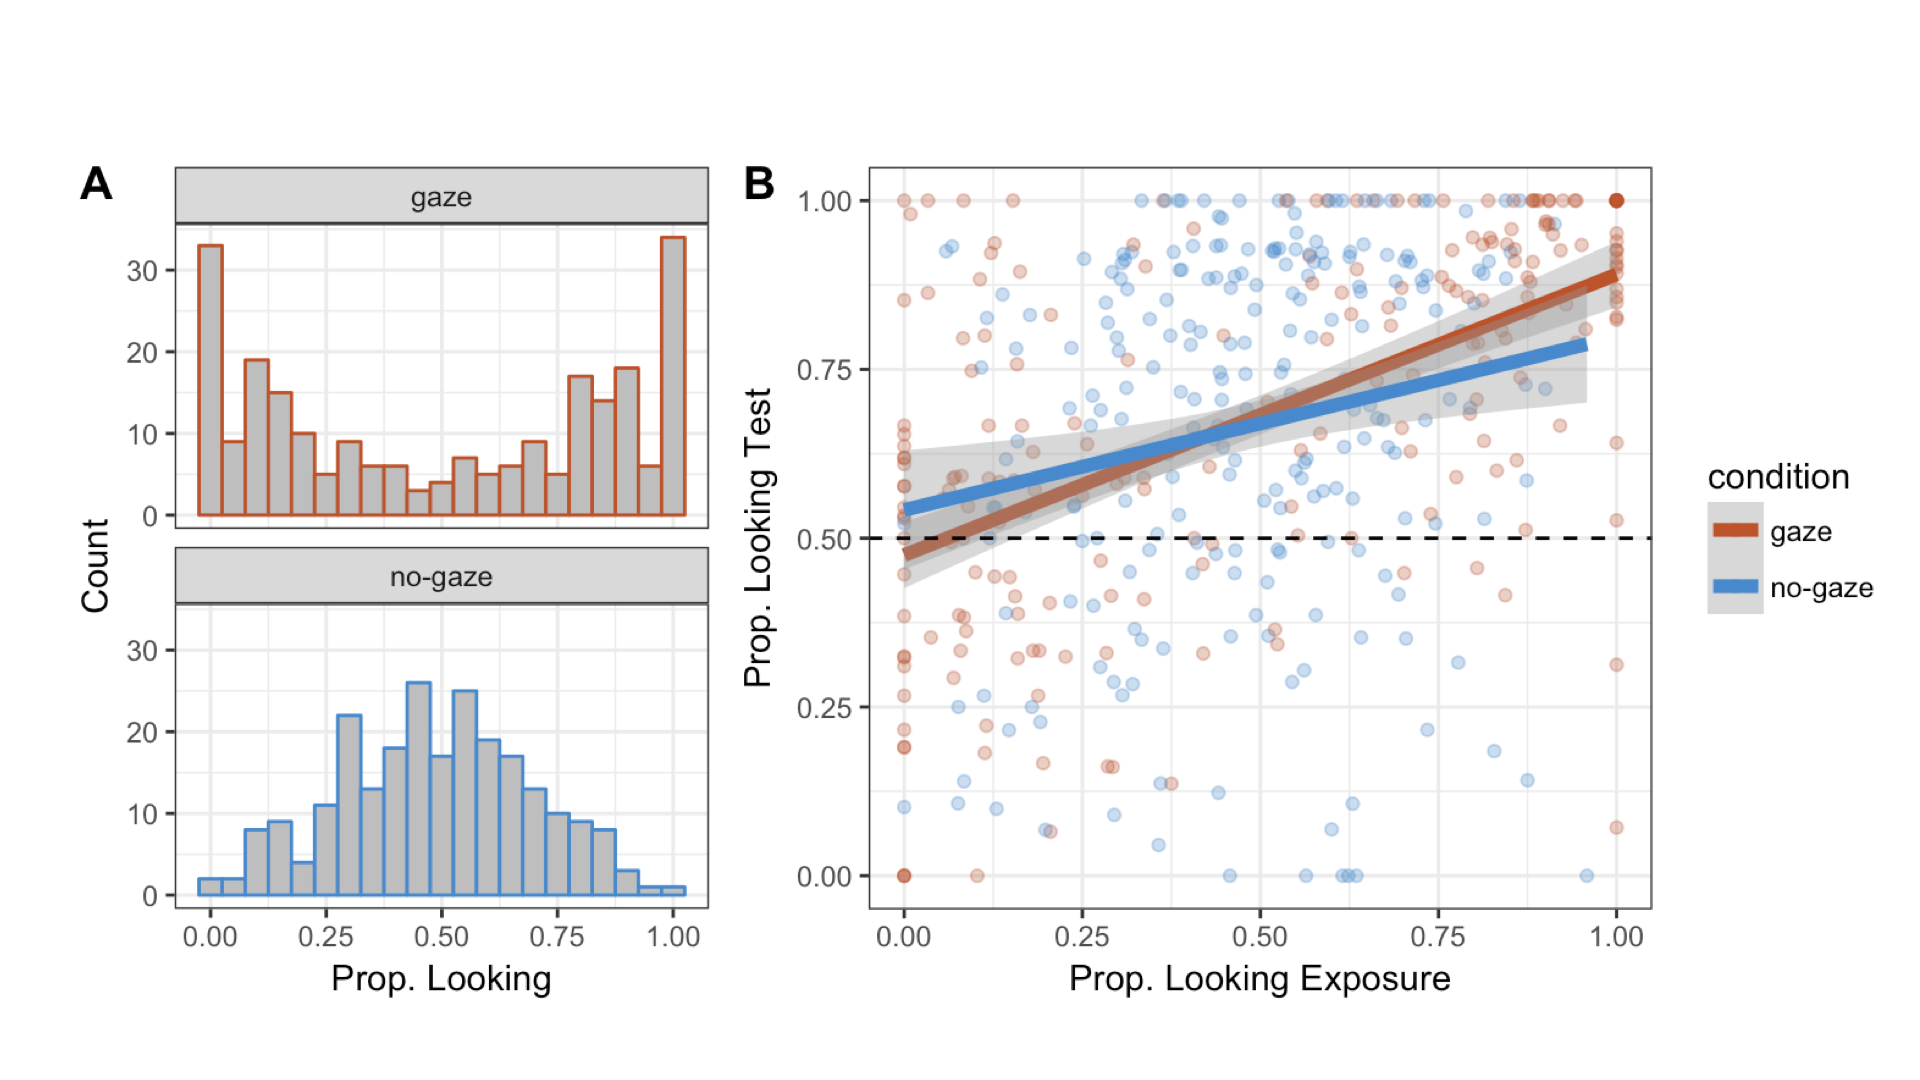
\includegraphics[width=0.9\linewidth]{/Users/kmacdonald/Documents/Projects/SPEED-ACC-NOVEL/writing/figures/gaze-xsit} 

}

\caption{Panel A shows adults' allocation of visual attention during exposure trials. Panel B shows adults' stronger memory for novel word-object links when there was a gaze cue present, even when they had fixated on the target objects for similar amounts of time during learning.}\label{fig:plot-e2}
\end{figure}

Learning occurred in both conditions. But when a social cue was present
during labeling, adults reliably used the cue (Figure XXX) and tended to
focus their attention on a single object (Figure XXX). In contrast,
people in the No-gaze condition tended to distribute their attention
more broadly. More time attending to the \enquote{kept} object during
exposure lead to better recall at test as shown by the linear
relationship between exposure and test trials (Figure XXX).

Critically, the presence of gaze modulated the relationship between
visual attention on exposure trials and test performance: that is, when
eye gaze cued adults' visual attention, they showed stronger memory for
the word-object link compared to when a gaze cue was absent (Figure
XXX). These data provide evidence that social information does more than
modulate how people allocate their visual attention; instead, social
contexts can change the strength of inferences that people make during
cross-situational word learning.

\hypertarget{limitations}{%
\subsubsection{Limitations}\label{limitations}}

There were several key limitations of our pilot study. First, we chose
to start the liguistic stimulus as soon as the images and the speaker
appeared on the screen (i.e., at trial onset). This made it difficult to
analyze the timing and accuracy of first shifts decisions away from the
speaker and to the objects. Second, this trial structure did not allow
us to measure decisions about visual fixation that occur before the
start of language comprehension while learners are first gathering
information about the visual world. Finally, the linguistic stimuli
consisted of sixteen pseudowords recorded by a speech synthesizer and
presented in isolation, thus removing any sentential context. Presenting
isolated words is unlikely to work with younger age groups and does not
allow us to separate decisions about fixations made during language
processing more broadly from decisions that occur after the onset of the
target noun -- a critical distinction for our modeling of the underlying
decision-making process.

\hypertarget{experiment-3}{%
\section{Experiment 3}\label{experiment-3}}

Experiment 3 was designed to address the limitations of Experiment
2.\footnote{See \url{https://osf.io/nfz85/} for a pre-registration of
  the analysis plan and predictions.} We modified the cross-situational
learning paradigm to parallel the design of Experiment 1. This allowed
us to use the analytic techniques developed for analyzing participants'
first gaze shifts to get a window onto children's decisions about visual
fixation as they get increased exposure to statistical information
within a social learning context.

\noindent We aim to answer the following specific research questions:

\begin{enumerate}
\def\labelenumi{\arabic{enumi}.}
\tightlist
\item
  How do decisions about where to allocate visual attention (speakers
  vs.~objects) change as a function of learning a new word?
\item
  How does the presence of a social cue to reference (eye gaze) change
  the dynamics of children's gaze patterns during object labeling?
\item
  What is the relationship between chidren's gaze patterns during object
  labeling and their memory of new words?
\end{enumerate}

\hypertarget{methods-2}{%
\subsection{Methods}\label{methods-2}}

\hypertarget{participants-2}{%
\subsubsection{Participants}\label{participants-2}}

\hypertarget{materials-2}{%
\subsubsection{Materials}\label{materials-2}}

\begin{figure}[!t]

{\centering 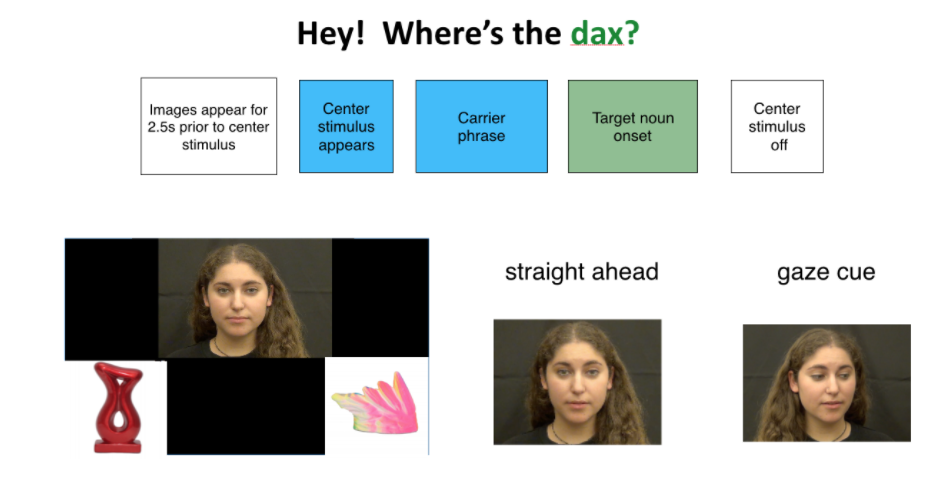
\includegraphics[width=0.9\linewidth]{/Users/kmacdonald/Documents/Projects/SPEED-ACC-NOVEL/writing/figures/speed_acc_novel_stim} 

}

\caption{Stimuli used in Experiment 3, including trial structure, fixation targets in the visual world, and the gaze cue manipulation.}\label{fig:speed-acc-novel-stimuli}
\end{figure}

\hypertarget{procedure-2}{%
\subsubsection{Procedure}\label{procedure-2}}

\hypertarget{results-and-discussion-2}{%
\subsection{Results and Discussion}\label{results-and-discussion-2}}

\hypertarget{general-discussion}{%
\section{General Discussion}\label{general-discussion}}

\newpage

\hypertarget{references}{%
\section{References}\label{references}}

\begingroup
\setlength{\parindent}{-0.5in}
\setlength{\leftskip}{0.5in}

\hypertarget{refs}{}
\leavevmode\hypertarget{ref-gabry2016rstanarm}{}%
Gabry, J., \& Goodrich, B. (2016). Rstanarm: Bayesian applied regression
modeling via stan. R package version 2.10. 0.

\leavevmode\hypertarget{ref-macdonald2018speed}{}%
MacDonald, K., Marchman, V., Fernald, A., \& Frank, M. C. (2018).
Children seek visual information during signed and spoken language
comprehension. \emph{Preprint PsyArXiv}.

\leavevmode\hypertarget{ref-macdonald2017social}{}%
MacDonald, K., Yurovsky, D., \& Frank, M. C. (2017). Social cues
modulate the representations underlying cross-situational learning.
\emph{Cognitive Psychology}, \emph{94}, 67--84.

\leavevmode\hypertarget{ref-maris2007nonparametric}{}%
Maris, E., \& Oostenveld, R. (2007). Nonparametric statistical testing
of eeg-and meg-data. \emph{Journal of Neuroscience Methods},
\emph{164}(1), 177--190.

\leavevmode\hypertarget{ref-vandekerckhove2007fitting}{}%
Vandekerckhove, J., \& Tuerlinckx, F. (2007). Fitting the ratcliff
diffusion model to experimental data. \emph{Psychonomic Bulletin \&
Review}, \emph{14}(6), 1011--1026.

\leavevmode\hypertarget{ref-wiecki2013hddm}{}%
Wiecki, T. V., Sofer, I., \& Frank, M. J. (2013). HDDM: Hierarchical
bayesian estimation of the drift-diffusion model in python.
\emph{Frontiers in Neuroinformatics}, \emph{7}, 14.

\endgroup


\end{document}
